In this section, we will provide a formal analysis of the system using the Alloy language. Alloy is a lightweight formal specification language that allows us to model the system's structure and behavior and verify the correctness of the system's design. The Alloy model will be used to verify the consistency of the system's requirements and to identify potential design flaws or inconsistencies of the Student\&Company platform. \\
First we will provide the code used to generate the model, broken down into tree main parts: the signature, the facts, and the assertion. Each part will be explained through comments present in the code itself. We will also provide a visual representation of the model generated by the code and it's evolution thought time as the model represents a dynamic system.
Finally, we will provide a discussion of the results obtained from the analysis and the potential implications for the system's design and implementation.
We decided to use Alloy to provide a formal analysis of the system Recommendation and Interview Process as they are the most complex part of the system and the one that could benefit the most from a formal correctness verification.

\subsection{Signatures}
The signature part of the code defines the different entities present in the system and their relationships. In this case, we will define the main entities of S\&C such as Students, Companies, Universities, InternshipsOffer, Recommendation, and Interview. 
\lstinputlisting[language=alloy]{Latex/Signatures.txt}
% \begin{verbatim}
% sig Email, VatNumber, CV{}{
%     //No Email, VatNumber or CV can be created without an associated user
%     Email = User.userEmail
%     VatNumber = (Company.companyVatNumber + University.universityVatNumber)
%     CV = Student.cv
% }
% abstract sig User {
%     userEmail: one Email,
% }
% sig Student extends User {
%     enrolledIn: one University,
%     cv: lone CV,
%     recommendations: set Recommendation,
%     spontaneousApplications: set SpontaneousApplication
% }
% sig University extends User {
%     universityVatNumber: one VatNumber,
% }
% sig Company extends User {
%     companyVatNumber: one VatNumber,
%     offeredInternshipPosition: set InternshipsOffer,
% }
% sig InternshipsOffer{
%     recommendations: set Recommendation,
%     spontaneousApplications: set SpontaneousApplication
% }{
%     //A InternshipOffer exists only if a company has offered it
%     InternshipsOffer = Company.offeredInternshipPosition
% }
% /*
% Define the possible status of a Recommendation.
% - toBeAccepted represents a match by the Platform 
% - acceptedByStudent and acceptedByCompany are refer in the document as "PendingMatch"
% - acceptedMatch and rejectedMatch have the same definition as in the document
% */
% enum recommendationStatus{toBeAccepted, acceptedByStudent, acceptedByCompany, acceptedMatch, rejectedMatch}
% /*
% Define the possible status of a SpontaneousApplication.
% - toBeEvaluated represents the sending of a spontaneous application that has not been evaluated by the Company yet
% - acceptedApplication and rejectedApplication are the possible outcomes of the evaluation of a spontaneous application
% */
% enum spontaneousApplicantStatus{toBeEvaluated, acceptedApplication, rejectedApplication}
% /*
% Define the possible status of an Interview.
% - toBeSubmitted represents the creation of an interview that has not been submitted yet
% - submitted represents the submission of the interview
% - passed and failed are the possible outcomes of the interview
% */
% enum interviewStatus{toBeSubmitted, submitted, passed, failed}
% sig Recommendation{
%     matchedStudent: one Student,
%     matchedInternship: one InternshipsOffer,
%     var status: one recommendationStatus
% }{
%     //A recommendation exists only if a student and an internship have been matched
%     (InternshipsOffer.recommendations & Student.recommendations) = Recommendation
% }
% sig SpontaneousApplication{
%     spontaneousApplicant : one Student,
%     interestedInternshipOffer: one InternshipsOffer,
%     var status: one spontaneousApplicantStatus
% }{
%     //A spontaneous application exists only if a student has sent it
%     (SpontaneousApplication & Student.spontaneousApplications) = SpontaneousApplication
% }
% //The signature Interview is variable as it is created only when a Recommendation or a SpontaneousApplication is accepted
% var sig Interview{
%     var recommendation: lone Recommendation,
%     var spontaneousApplication: lone SpontaneousApplication,
%     var status: one interviewStatus
% }{
%     //An interview can only be assign to a recommendation or a spontaneous application
%     recommendation.status = acceptedMatch <=> !spontaneousApplication.status = acceptedApplication
%     one recommendation => no spontaneousApplication
%     one spontaneousApplication => no recommendation
% }
% \end{verbatim}
\subsection{Facts}
Facts represent the constraints that the system must respect and are always true in the model. For this application we defined facts such as the necessity of a Student to have a CV to be matched with an Internship or the different stage of evolution of an Internship Offer and Interview
\lstinputlisting[language=alloy]{Latex/Facts.txt}
% \begin{verbatim}
% // Two distinct interview cannot share the same reccomendation or spontaneous application
% fact interviewUniqueness{
%     always all i1, i2: Interview | i1 != i2 => ((i1.recommendation & i2.recommendation) = none) and ((i1.spontaneousApplication & i2.spontaneousApplication) = none)
% }
% //Ensure that VatNumbers and unique for Company and University
% fact UniqueVatNumber{
%     //The set of VatNumbers for companies and universities should be different from each other
%     Company.companyVatNumber & University.universityVatNumber = none
%     //Different companies and universities should have different vat numbers
%     all c1, c2: Company | c1 != c2 => c1.companyVatNumber != c2.companyVatNumber
%     all u1, u2: University | u1 != u2 => u1.universityVatNumber != u2.universityVatNumber
% }
% //Different Users shall have different emails
% fact UniqueEmailEndEnrollment{
%     all u1, u2: User | u1 != u2 => u1.userEmail != u2.userEmail
% }
% //All students shall be enrolled in a university
% fact StudentEnrolledInUniversity{
%     all s: Student | s.enrolledIn != none
% }
% //Different students shall have different CVs
% fact CurriculumUniqueness{
%     all s1, s2: Student | (s1 != s2 and s1.cv != none and s2.cv != none) => s1.cv != s2.cv
% }
% //Different companies shall have different offeredInternshipPositions
% fact UniqueInternshipOffer{
%     all c1, c2: Company | (c1 != c2 and c1.offeredInternshipPosition != none and c2.offeredInternshipPosition != none) => c1.offeredInternshipPosition != c2.offeredInternshipPosition
% }
% //Only a student with a Cv and a Company with an OfferedInternshipPosition can be matched.
% //Only a student with a Cv can send a spontaneous application
% fact StudentWithCVInteraction{
%     all r: Recommendation | r.matchedStudent.cv != none && r.matchedInternship != none
%     all s: SpontaneousApplication | s.spontaneousApplicant.cv != none && s.interestedInternshipOffer != none
% }
% //Define how one Recommendation differs from another Recommendation and similarly for SpontaneousApplications
% fact SingleApplicationSource{
%     all r1, r2: Recommendation | r1 != r2 => r1.matchedStudent != r2.matchedStudent or r1.matchedInternship != r2.matchedInternship 
%     all sa1, sa2: SpontaneousApplication | sa1 != sa2 => sa1.spontaneousApplicant != sa2.spontaneousApplicant or sa1.interestedInternshipOffer != sa2.interestedInternshipOffer
% }
% //Define the reflexive property Recommendation and SpontaneousApplication
% fact ApplicationReflexivity{
%     all r: Recommendation, i: InternshipsOffer | r in i.recommendations <=> r.matchedInternship = i
%     all r: Recommendation, s: Student | r in s.recommendations => r.matchedStudent = s
%     all sa: SpontaneousApplication, i: InternshipsOffer | sa in i.spontaneousApplications <=> sa.interestedInternshipOffer = i
%     all sa: SpontaneousApplication, s: Student | sa in s.spontaneousApplications => sa.spontaneousApplicant = s
% }
% //An Application is unique and cannot be shared between two different Students or InternshipOffers
% fact ApplicationUniqueness{
%     all i1, i2: InternshipsOffer | i1 != i2 =>  ((i1.recommendations & i2.recommendations) = none)
%     all sa1, sa2: SpontaneousApplication | sa1 != sa2 =>  ((sa1.interestedInternshipOffer & sa2.interestedInternshipOffer) = none)
% }
% //Define the initial status of a Recommendation and a SpontaneousApplication
% fact initAcceptance {
%     Recommendation.status = toBeAccepted
%     SpontaneousApplication.status = toBeEvaluated
% }
% //Constraints that define the evolution of the status of a Recommendation
% fact RecommendationEvolutionRules{
%     //A Match need to be accepted by both parties before it can be considered accepted. It can't become accepted in one-step
%     all r: Recommendation | always ((r.status = toBeAccepted) => (r.status' != acceptedMatch))
%     //A party cannot retract its acceptance of a match. Once accepted, it remains accepted.
%     all r: Recommendation | always ((r.status = acceptedByStudent) => (r.status' != acceptedByCompany and r.status' != toBeAccepted))
%     all r: Recommendation | always ((r.status = acceptedByCompany) => (r.status' != acceptedByStudent and r.status' != toBeAccepted))
%     //Rejected and accepted matches remain rejected and accepted forever
%     all r: Recommendation | always ((r.status = rejectedMatch) => always (r.status = rejectedMatch))
%     all r: Recommendation | always ((r.status = acceptedMatch) => always (r.status = acceptedMatch))
% }
% //Constraints that define the evolution of the status of a SpontaneousApplication
% fact SpontaneousApplicationEvolutionRules{
%     always all sa: SpontaneousApplication | (sa.status = toBeEvaluated) => ((sa.status' = acceptedApplication) or (sa.status' = rejectedApplication) or (sa.status' = toBeEvaluated))
%     //Once a spontaneous application has been accepted or rejected, it cannot change its status
%     all sa: SpontaneousApplication | always ((sa.status = acceptedApplication) => always (sa.status = acceptedApplication))
%     all sa: SpontaneousApplication | always ((sa.status = rejectedApplication) => always (sa.status = rejectedApplication))
    
% }
% //Here the Interviews are created and for now the starting status is toBeSubmitted
% fact InterviewIFRecommendationAccepted{
%     always all r: Recommendation | ((r.status = acceptedMatch) => (one i: Interview |  i.recommendation = r ))
%     always all sa: SpontaneousApplication | ((sa.status = acceptedApplication) => (one i: Interview | i.spontaneousApplication = sa))
%     always all i: Interview, r:Recommendation | ((i.recommendation = r) => always (i.recommendation = r))
%     always all i: Interview, r:SpontaneousApplication | ((i.spontaneousApplication = r) => always (i.spontaneousApplication = r))
%     always (all i: Interview | once (i.status = toBeSubmitted))
% }
% fact InterviewStatusEvolution{
%     // If interview is submitted, then sometime in the past it had to be toBeSubmitted
%     always all i: Interview | always ((i.status = submitted) => once (i.status = toBeSubmitted and i.status' = submitted)) 
%     // If interview is failed, then sometime in the past it had to be submitted
%     always all i: Interview | always ((i.status = failed) => once (i.status = submitted and i.status' = failed))
%     // If interview is passed, then sometime in the past it had to be submitted
%     always all i: Interview | always ((i.status = passed) => once (i.status = submitted and i.status' = passed)) 
%     always all i: Interview | always ((i.status = submitted) => after always (i.status != toBeSubmitted))
%     always all i: Interview | always ((i.status = passed) => after always (i.status != submitted))
%     always all i: Interview | always ((i.status = failed) => after always (i.status != submitted))
%     always all i: Interview | always ((i.status' != toBeSubmitted) => once (i.status = toBeSubmitted))
% }
% \end{verbatim}
\subsection{Assertions}
Assertions are the properties that we want to verify in the model to avoid unwanted behavior by the Platform. For this scenario we verified different aspects such as the necessity of both Student and Company to accept a Match before starting an Interview or the fact that only a student with a CV uploaded to the platform can have completed an interview.

\lstinputlisting[language=alloy]{Latex/Assertions.txt}
% \begin{verbatim}
% //A function that returns the company that has offered a specific InternshipsOffer
% fun FindInternshipPositionCompany[i: InternshipsOffer]: lone Company {
%     { c: Company | i in c.offeredInternshipPosition }
% }
% //If a student has no CV, then it cannot be matched with a recommendation or send a spontaneous application
% //If a company has no offeredInternshipPosition, then it cannot be matched with a recommendation
% assert NoInfoProvided{
%     all s: Student, r: Recommendation | (s.cv = none) => (r.matchedStudent != s)
%     all s: Student, sa: SpontaneousApplication | (s.cv = none) => (sa.spontaneousApplicant != s)
%     all c: Company, r: Recommendation | (c.offeredInternshipPosition = none) => (FindInternshipPositionCompany[r.matchedInternship] != c)
% }
% //For a recommendation to be accepted, both the student and the company need to accept it
% //For a spontaneous application to be accepted, it needs to be evaluated
% assert BothPartyNeedToAct{
%     always all r: Recommendation | (r.status' = acceptedMatch) => (r.status = acceptedByStudent or r.status = acceptedByCompany or r.status = acceptedMatch)
%     always all sa: SpontaneousApplication | (sa.status' = acceptedApplication) => (sa.status = toBeEvaluated or sa.status = acceptedApplication)
% }
% //If a student has multiple recommendations, then the recommendations are for different InternshipOffers
% //If a InternshipOffer has multiple recommendations, then the students recommended are different
% assert UniqueRecommendation{
%     all s: Student, r1, r2: Recommendation | (r1 != r2 and r1.matchedStudent = s and r2.matchedStudent = s) => r1.matchedInternship != r2.matchedInternship
%     all i: InternshipsOffer, r1, r2: Recommendation | (r1 != r2 and r1.matchedInternship = i and r2.matchedInternship = i) => r1.matchedStudent != r2.matchedStudent
% }
% //Two companies cannot offer the same InternshipOffer
% assert internshipsOfferUniqueness{
%     all c1, c2: Company | (c1 != c2 and c1.offeredInternshipPosition != none and c2.offeredInternshipPosition != none) => c1.offeredInternshipPosition != c2.offeredInternshipPosition
% }
% //Two students cannot have the same CV
% assert CVUniqueness{
%     all s1, s2: Student | (s1 != s2 and s1.cv != none and s2.cv != none) => s1.cv != s2.cv
% }
% //An interview can be assigned to a recommendation or a spontaneous application only if they have been accepted
% assert InterviewAssignment{
%     always all i: Interview | (i.recommendation.status = acceptedMatch or i.spontaneousApplication.status = acceptedApplication)
% }
% //An interview can be assigned only to a student with a CV
% assert StudentWithInterviewHasCV{
%     //(A <=> !B) equivalent to (A = !B and B = !A) equivalent to (A XOR B)
%     always all i: Interview | (i.recommendation.matchedStudent.cv != none) <=> !(i.spontaneousApplication.spontaneousApplicant.cv != none)
% }
% \end{verbatim}

\subsection{Model Visualization}
The following model was obtained with the following run:
\lstinputlisting[language=alloy]{Latex/Run.txt}
% \begin{verbatim}
%         run {} for 7 but exactly 3 Recommendation, exactly 2 Company, exactly 3 Student, exactly 2 University, exactly 2 SpontaneousApplication, exactly 4 InternshipsOffer, exactly 2 CV, exactly 10 steps 
% \end{verbatim}
and represent a typical evolution of the system composed where it is possible to see the different entities, their relationships and the evolution of the status of such entities like Recommendation and Interview
Such parameter for the run command were chosen to provide a clear and readable model that can be easily understood by the reader, but they can be easily modified to provide a more detailed or more general model. 

\begin{figure}[h]
    \centering
    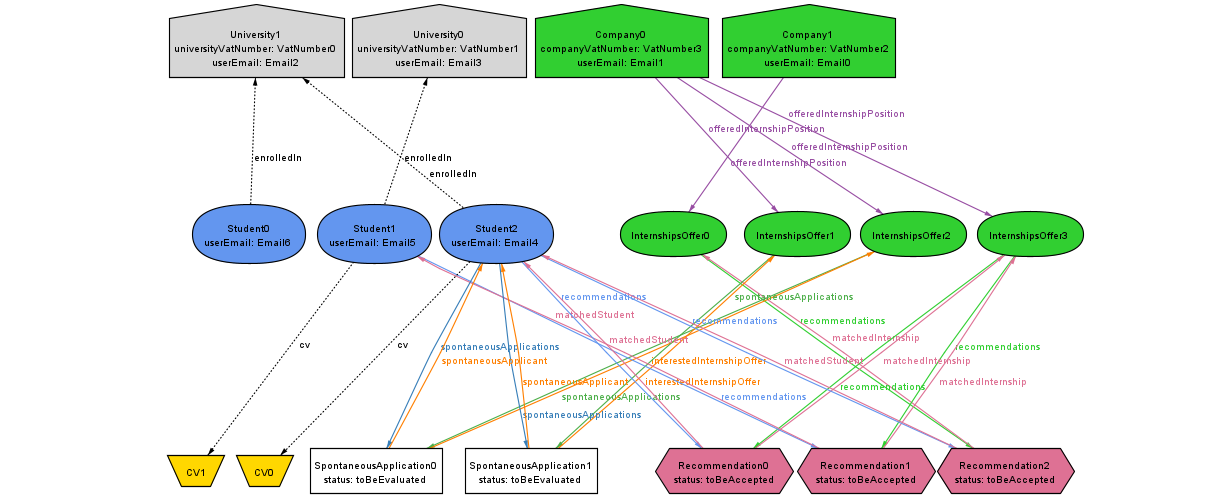
\includegraphics[width=0.9\textwidth]{Alloy/AlloyImage/0.png}
    \caption{Step 0: All Recommendations and Spontaneous Applications have been sent but have not yet been evaluated.}
    \label{fig:ALIMG0}
\end{figure}
\begin{figure}[h]
    \centering
    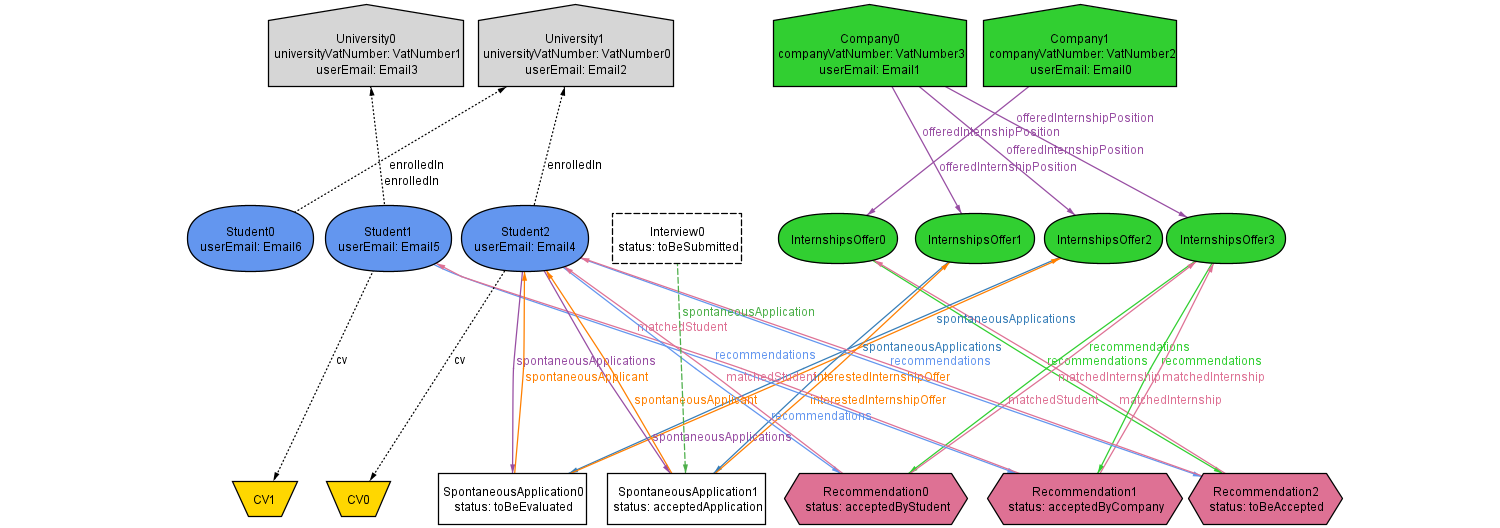
\includegraphics[width=0.9\textwidth]{Alloy/AlloyImage/1.png}
    \caption{Step 1: A Spontaneous Application has been accepted, and an Interview has been created}
    \label{fig:ALIMG1}
\end{figure}
\begin{figure}[h]
    \centering
    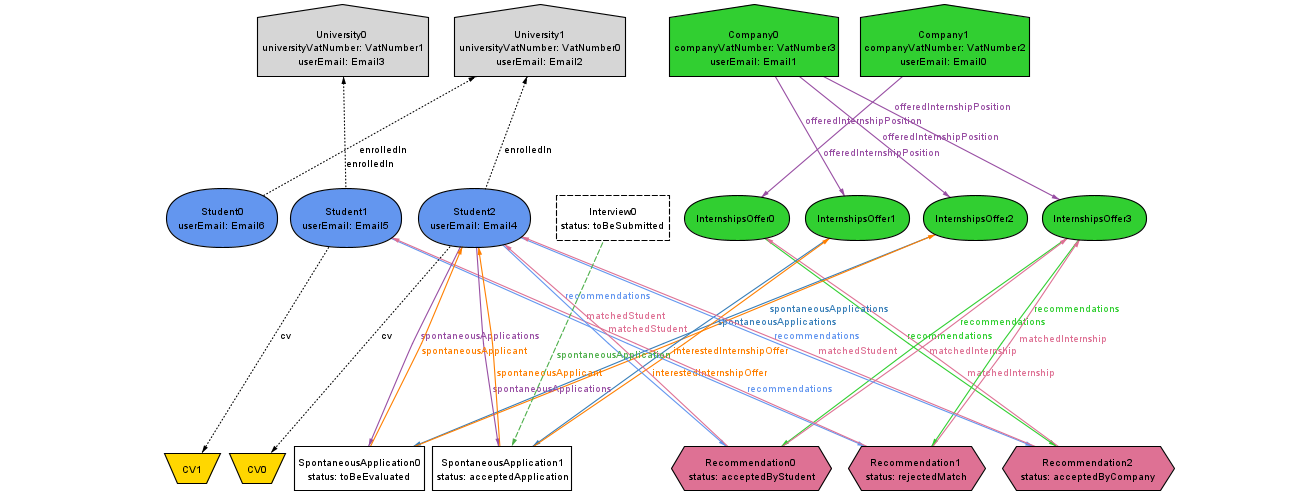
\includegraphics[width=0.9\textwidth]{Alloy/AlloyImage/2.png}
    \caption{Step 2: A Recommendation has been rejected by one of the party}
    \label{fig:ALIMG2}
\end{figure}
\begin{figure}[h]
    \centering
    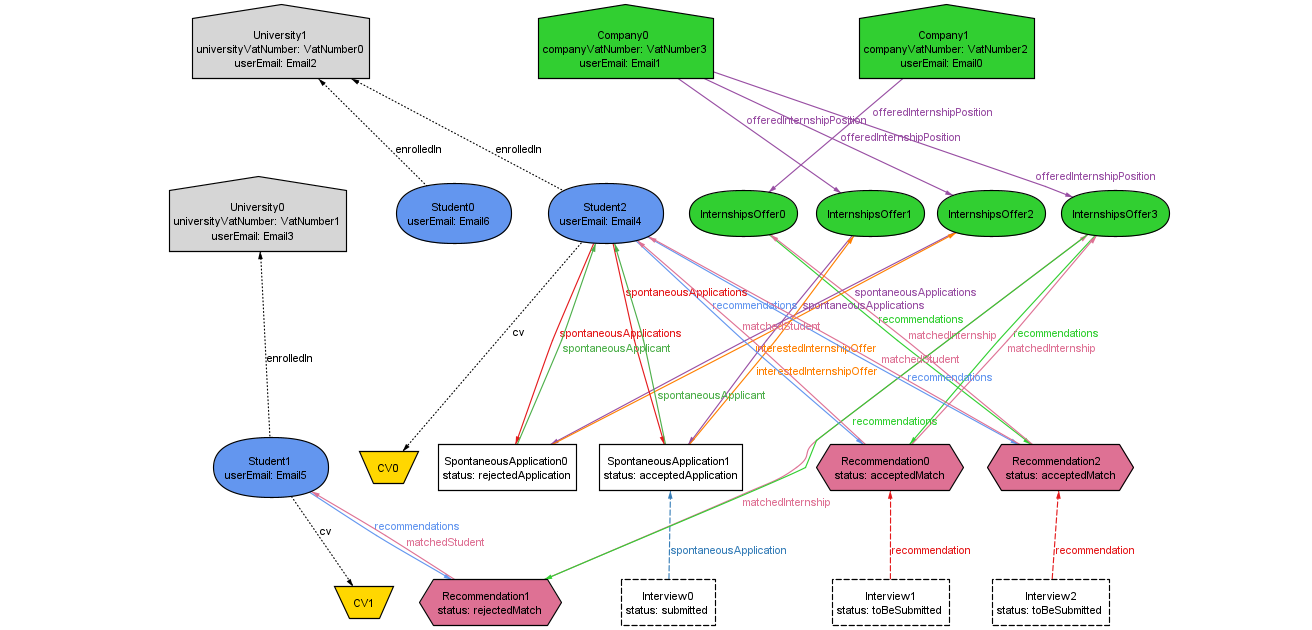
\includegraphics[width=0.9\textwidth]{Alloy/AlloyImage/3.png}
    \caption{Step 3: Another Spontaneous Application has been accepted, and the first Interview has been sent. }
    \label{fig:ALIMG3}
\end{figure}

